\newpage % Nova página
\clearpage % Finaliza a página atual

\section{Introdução} % Inicia a seção "Introdução"
\subsection{subCap 1}

% Exemplo Citação
Exemplo citação \cite{Mussoi} 

% Exemplo Equação
Exemplo de Equação:
\myequation{Z_C(\omega) = \frac{1}{\omega \cdot C}}{eq:Exemplo}{Impedância de um capacitor}{$\Omega$}
Exemplo chamada de referencia da Equação~\ref{eq:Exemplo}


% Exemplo Codigo
Exemplo codigo:
\begin{lstlisting}[language=Python]
def hello_world():
    print("Hello, World!")
\end{lstlisting}

% Exemplo Circuito
Exemplo Circuito:
\begin{figure}[H]
\centering
\caption{Exemplo Circuito}
\centering
\begin{circuitikz} \draw 
    (0,0) node[above]{I/O Pin} to[short, o-] ++(2,0)
    (2,0) to[push button] (2,-2) 
    (2,0) to[R, l_=10k\ohm] (4,0)
    (4,0) to[short] (4,2)
    (2,-2) to[short] (2,-3)
    (4,2) node[vcc]{+5V} 
    (2,-3) node[ground]{}
    (2,-3) node[anchor=west] {0V}
    ;
    \end{circuitikz} 
\centering 
\vspace{0.2cm} \\
Fonte: Autor.
\label{fig:ExemploCircuito}
\end{figure}

Exemplo chamada de referencia do circuito~\ref{fig:ExemploCircuito}.

% Exemplo Imagem
\begin{figure}[H]
\centering
\caption{Exemplo Imagem}
\centering

\includegraphics[scale = .5]{Imagens/Capa/01_Instituto.png}
\centering 
\vspace{0.2cm} \\
Fonte: Autor.
\label{fig:ExemploFigura}
\end{figure}

Exemplo chamada de referencia da figura~\ref{fig:ExemploFigura}.

% Exemplo Gráfico
\begin{figure}[H]
\centering
\caption{Exemplo Gráfico}
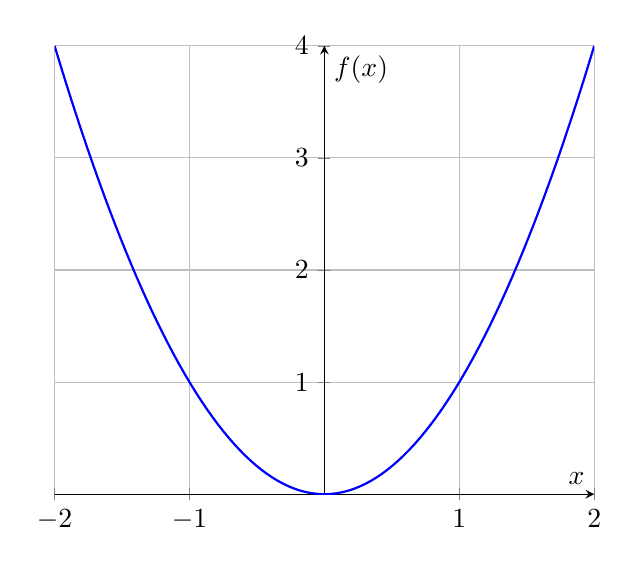
\begin{tikzpicture}
\begin{axis}[
    axis lines = middle,
    xlabel = {$x$},
    ylabel = {$f(x)$},
    % title = {Gráfico de $f(x) = x^2$},
    grid = both,
]
\addplot[
    domain=-2:2,
    samples=100,
    thick,
    blue
]
{x^2};
\end{axis}
\end{tikzpicture}
\centering 
\vspace{0.2cm} \\
Fonte: Autor.
\label{fig:ExemploGráfico}
\end{figure}

Exemplo chamada de referencia da figura~\ref{fig:ExemploGráfico}.

% Exemplo Tabela
\begin{table}[H]
\centering
\caption{Exemplo Tabela}
\begin{tabular}{|c|c|}
\hline
\textbf{Texto1} & \textbf{Texto 2} \\ \hline
Teste1 & Teste2 \\ \hline
\end{tabular}
\vspace{0.25cm} \\
Fonte: Autor.
\label{tab:ExemploTabela}
\end{table}

Exemplo chamada de referencia da tabela~\ref{tab:ExemploTabela}.


\par Exemplo do uso do SI \SI{6,660}{\hertz}, \SI{100}{\hertz}, \SI{0,5}{\volt} e \SI{3,5}{\volt}.
